\documentclass[journal,12pt,twocolumn]{IEEEtran}

\usepackage{setspace}
\usepackage{textcomp,gensymb}
\singlespacing
\usepackage[cmex10]{amsmath}
\usepackage{enumerate}
\usepackage{amsmath}

\usepackage{amsthm}

\usepackage{mathrsfs}
\usepackage{txfonts}
\usepackage{stfloats}
\usepackage{bm}
\usepackage{cite}
\usepackage{cases}
\usepackage[caption=false]{subfig}

\usepackage{longtable}
\usepackage{multirow}



\usepackage{mathtools}
\usepackage{steinmetz}
\usepackage{tikz}


\usepackage{verbatim}
\usepackage{tfrupee}
\usepackage[breaklinks=true]{hyperref}
\usepackage{graphicx}
\usepackage{tkz-euclide}
\usepackage[rightcaption]{sidecap}


\usepackage{graphicx} 
\graphicspath{ {images/} }


\usetikzlibrary{calc,math}
\usepackage{listings}
    \usepackage{color}                                            %%
    \usepackage{array}                                            %%
    \usepackage{longtable}                                        %%
    \usepackage{calc}                                             %%
    \usepackage{multirow}                                         %%
    \usepackage{hhline}                                           %%
    \usepackage{ifthen}                                           %%
    \usepackage{lscape}     


\DeclareMathOperator*{\Res}{Res}
\DeclareUnicodeCharacter{2212}{-}

\renewcommand\thesection{\arabic{section}}
\renewcommand\thesubsection{\thesection.\arabic{subsection}}
\renewcommand\thesubsubsection{\thesubsection.\arabic{sub-subsection}}

\renewcommand\thesectiondis{\arabic{section}}
\renewcommand\thesubsectiondis{\thesectiondis.\arabic{subsection}}
\renewcommand\thesubsubsectiondis{\thesubsectiondis.\arabic{sub-subsection}}


\hyphenation{op-ti-cal net-works semi-conduc-tor}
\def\inputGnumericTable{}                                 %%

\lstset{
%language=C,
frame=single, 
breaklines=true,
columns=fullflexible
}

\begin{document}


\newtheorem{theorem}{Theorem}[section]
\newtheorem{problem}{Problem}
\newtheorem{proposition}{Proposition}[section]
\newtheorem{lemma}{Lemma}[section]
\newtheorem{corollary}[theorem]{Corollary}
\newtheorem{example}{Example}[section]
\newtheorem{definition}[problem]{Definition}

\newcommand{\BEQA}{\begin{eqnarray}}
\newcommand{\EEQA}{\end{eqnarray}}
\newcommand{\define}{\stackrel{\triangle}{=}}
\bibliographystyle{IEEEtran}
\raggedbottom
\setlength{\parindent}{0pt}
\providecommand{\mbf}{\mathbf}
\providecommand{\pr}[1]{\ensuremath{\Pr\left(#1\right)}}
\providecommand{\qfunc}[1]{\ensuremath{Q\left(#1\right)}}
\providecommand{\sbrak}[1]{\ensuremath{{}\left[#1\right]}}
\providecommand{\lsbrak}[1]{\ensuremath{{}\left[#1\right.}}
\providecommand{\rsbrak}[1]{\ensuremath{{}\left.#1\right]}}
\providecommand{\brak}[1]{\ensuremath{\left(#1\right)}}
\providecommand{\lbrak}[1]{\ensuremath{\left(#1\right.}}
\providecommand{\rbrak}[1]{\ensuremath{\left.#1\right)}}
\providecommand{\cbrak}[1]{\ensuremath{\left\{#1\right\}}}
\providecommand{\lcbrak}[1]{\ensuremath{\left\{#1\right.}}
\providecommand{\rcbrak}[1]{\ensuremath{\left.#1\right\}}}
\theoremstyle{remark}
\newtheorem{rem}{Remark}
\newcommand{\sgn}{\mathop{\mathrm{sgn}}}
\providecommand{\res}[1]{\Res\displaylimits_{#1}} 
%\providecommand{\norm}[1]{\lVert#1\rVert}
\providecommand{\mtx}[1]{\mathbf{#1}}
\providecommand{\fourier}{\overset{\mathcal{F}}{ \rightleftharpoons}}
\providecommand{\hilbert}{\overset{\mathcal{H}}{ \rightleftharpoons}}
\providecommand{\system}{\overset{\mathcal{H}}{ \longleftrightarrow}}
	\newcommand{\solution}[2]{\textbf{Solution:}{#1}}
%\newcommand{\cosec}{\,\text{cosec}\,}
\providecommand{\dec}[2]{\ensuremath{\overset{#1}{\underset{#2}{\gtrless}}}}
\newcommand{\myvec}[1]{\ensuremath{\begin{pmatrix}#1\end{pmatrix}}}
\newcommand{\mydet}[1]{\ensuremath{\begin{vmatrix}#1\end{vmatrix}}}
\numberwithin{equation}{subsection}
\makeatletter
\@addtoreset{figure}{problem}
\makeatother
\let\StandardTheFigure\thefigure
\let\vec\mathbf
\renewcommand{\thefigure}{\theproblem}
\def\putbox#1#2#3{\makebox[0in][l]{\makebox[#1][l]{}\raisebox{\baselineskip}[0in][0in]{\raisebox{#2}[0in][0in]{#3}}}}
     \def\rightbox#1{\makebox[0in][r]{#1}}
     \def\centbox#1{\makebox[0in]{#1}}
     \def\topbox#1{\raisebox{-\baselineskip}[0in][0in]{#1}}
     \def\midbox#1{\raisebox{-0.5\baselineskip}[0in][0in]{#1}}
\title{Assignment 5}
\author{Prabhath Chellingi - CS20BTECH11038}
\maketitle
\newpage
\bigskip
\renewcommand{\thefigure}{\theenumi}
\renewcommand{\thetable}{\theenumi}

Download all python codes from 
\begin{lstlisting}

\end{lstlisting}

and latex-tikz codes from
\begin{lstlisting}

\end{lstlisting}

\section{Problem}

$(GATE(EC)2013-26Q)$ Let $U$ and $V$ be two independent zero mean Gaussian random variables of variances $\frac{1}{4}$ and $\frac{1}{9}$ respectively. The probability $\pr{3V\geq2U }$ is
\begin{enumerate}[(A)]
    \item $4/9$
    \item $1/2$
    \item $2/3$
    \item $5/9$
\end{enumerate}

\section{Solution}

$U$ and $V$ are independent random variables,
\begin{align}
    V\sim N\brak{0,\frac{1}{9}}
\end{align}
\begin{align}
    U\sim N\brak{0,\frac{1}{4}}
\end{align}
Let,
\begin{align}
    Z=3V-2U
\end{align}
\begin{align}
    Z\sim N\brak{0,9\times\frac{1}{9}+4\times\frac{1}{4}}
\end{align}
\begin{align}
    Z\sim N\brak{0,2}
\end{align}
For $Z$, $\mu=0$, and $\sigma^2=2$.

By Gaussian Distribution,

$PDF$ of $Z$,
\begin{align}
    f_Z(z)=\frac{1}{\sqrt{2\pi}\sigma}e^{-\frac{\brak{z-\mu}^2}{2\sigma^2}}
\end{align}
\begin{align}
    f_Z(z)=\frac{1}{2\sqrt{\pi}}e^{-\frac{z^2}{4}}
\end{align}
\begin{figure}[h!]
    \centering
    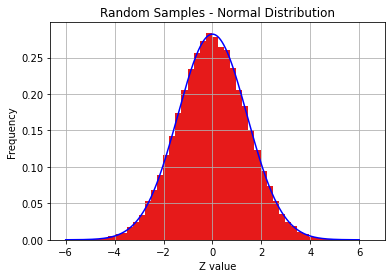
\includegraphics[width=\columnwidth]{Figure.png}
    \caption{Plot of of distribution function}
    \label{fig:plot}
\end{figure}
\begin{align}
    \pr{Z\geq0}=\int\limits_0^{\infty}f_Z(z)dz
\end{align}
\begin{align}
    \pr{Z\geq0}=\frac{1}{2}\int\limits_{-\infty}^{\infty}\frac{1}{2\sqrt{\pi}}e^{-\frac{z^2}{4}}dz
\end{align}
\begin{align}
    \pr{Z\geq0}=\frac{1}{2}\frac{1}{2\sqrt{\pi}}\int\limits_{-\infty}^{\infty}e^{-\frac{z^2}{4}}dz
\end{align}
\begin{align}
    \pr{Z\geq0}=\frac{1}{2}\frac{1}{2\sqrt{\pi}}\brak{\sqrt{4\pi}}
\end{align}
\begin{align}
    \pr{Z\geq0}=\frac{1}{2}
\end{align}
\begin{align}
    \pr{3V-2U\geq0}=\frac{1}{2}
\end{align}
\begin{align}
    \pr{3V\geq2U}=\frac{1}{2}
\end{align}
Option (B) is correct.

\end{document}